\subsection{Resumen del proyecto}
Solar Link es un administrador inteligente de energía eléctrica (Smart Grid) que busca maximizar el uso de energías renovables. A través de paneles solares, y con un sistema inteligente, alimentar todo el consumo hogareño posible con energía solar, “switcheando” las líneas de la casa (ejemplo iluminación, tomacorrientes) entre la línea eléctrica del proveedor (edesur p/ej) y la alimentación renovable.\\

Nuestro proyecto es, en esencia, una combinación de los desarrollos en ingeniería eléctrica más reciente (con un hincapié en renovables), y nuestros conocimientos de electrónica e informática. Además, Solar Link estará vinculado a una app y una web para que el usuario pueda ver, controlar y configurar su consumo.\\

Por ejemplo, en una casa el router, la televisión u otros electrodomésticos de uso común que poseen un bajo consumo, pueden ser alimentados con una red solar económica sin problema, pero si a estos consumos se les suman electrodomésticos de alto consumo como lo pueden ser microondas, pavas eléctricas, aires acondicionados, ya no se podrían alimentar por este medio.\\

Por eso, la propuesta de Solar Link es medir constantemente el consumo hogareño, y monitorear si el consumo es lo suficientemente bajo como para ser alimentado por una red de energía solar, o si es demasiado alto como para esta. Dependiendo de esto, el sistema elegirá si la alimentación de la casa será de energía solar o del proveedor de energía eléctrica convencional, conmutando entre estas dos fuentes de energía.\\

En caso de cortes de suministro de luz, Solar Link puede encargarse de lo esencial de la casa que haga falta alimentar, siempre que esté en su margen de funcionamiento.\\

Por otro lado la aplicación web, vinculada con el tablero del usuario, puede mostrarte el consumo hogareño en tiempo real, cuánto consumiste de cada origen y ahorraste en el último tiempo, cuánto significa eso de precio en la factura de luz. También predicciones de la eficiencia de los paneles según el clima presente y futuro. Por último configurar el tablero según la cantidad de baterías o paneles solares y su capacidad.\\

Por último, el proyecto plantea ser modular y versátil, de forma tal que el tablero puede trabajar con cualquier cantidad de paneles o baterías que se le suministren: Solar Link no está limitado sólo a una fuente de energía solar. Aunque el enfoque de nuestro proyecto es aprovechar este tipo de energía, el sistema permite aprovechar también cualquier tipo de fuente: desde una red de proveedor extra, pasando por cosas como un grupo electrógeno, y hasta otras fuentes renovables; biogas, eólica, etc.\\

\subsection{¿Por qué Solar Link?}

\subsubsection{El aspecto de energías no renovables}

Las principales fuentes de energía con las que cuenta hoy el mundo, petróleo, gas natural y carbón mineral, son de carácter no renovable o convencional; es decir que a medida que se van consumiendo disminuyen sus reservas sin posible reposición, salvo que se descubran nuevos yacimientos.\\

Este sector de energías convencionales sigue teniendo un papel protagónico en la matriz energética mundial, producto de un mercado con muchos años de desarrollo tecnológico, con un gran capital hundido en infraestructura, costos competitivos y con porcentajes de rendimiento y de potencia firme superiores a las renovables. Sin embargo, el consumo de combustibles de origen fósil tiene un efecto muy negativo para el medio ambiente, ya que el dióxido de carbono que se produce por su combustión es el principal constituyente de lo que se conoce como gases de efecto invernadero, principales responsables del calentamiento global.\\

Las consecuencias de este efecto son, por ejemplo, el aumento de las temperaturas, los picos de temperaturas extremos, que han venido manifestándose en los últimos años. Es por ello, que las emisiones globales de carbono continúan aumentando, lo que indica la necesidad de un conjunto integral de medidas políticas para lograr la reducción sustancial de las emisiones de carbono.\\

\begin{figure}[H]
    \centering
    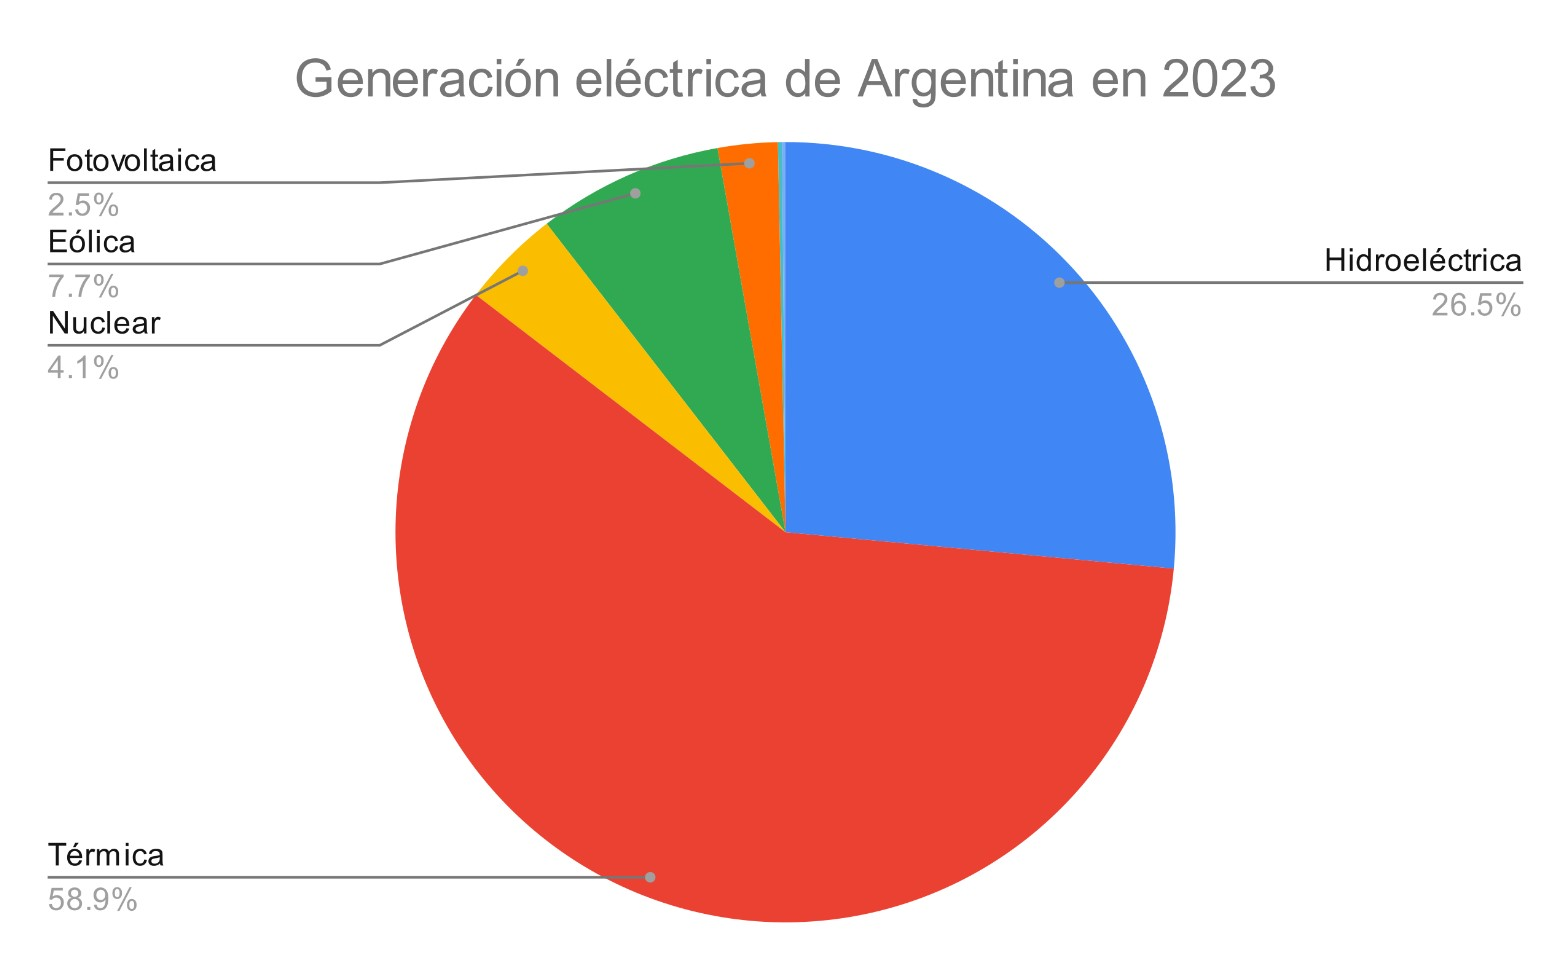
\includegraphics[width=0.85\linewidth]{Intro/Screenshot_20.jpg}
    \caption{Matriz de generación energética en Argentina}
    \label{fig:matriz-energias}
\end{figure}

En Argentina, casi el 60\% de la energía producida y distribuida en el país son de carácter no renovable. La visión de Solar Link es aportar a que esta brecha vaya disminuyendo hasta su exterminacion, volviendo a las energías renovables cabecillas en la generacion de energia. \\

\subsubsection{El aspecto de la energía solar}
Considerando el contexto geográfico y ambiental del país en cuanto a energías renovables, Argentina es un escenario ideal para aplicarlas. Sin embargo, al ver la matriz energética eléctrica de nuestro país, esto no se aprovecha.

\begin{figure}[H]
\centering
\begin{subfigure}{0.4\textwidth}
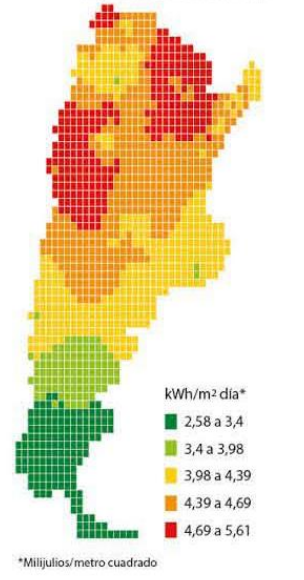
\includegraphics[width=1\linewidth]{Intro/Screenshot_1.png} 
\caption{Zonas del país con mayor \\promedio de intensidad de \\radiación solar}
\end{subfigure}
\begin{subfigure}{0.4\textwidth}
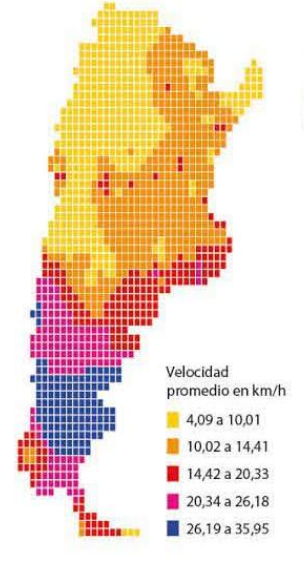
\includegraphics[width=1\linewidth]{Intro/Screenshot_2.png}
\caption{Zonas del país con mayor \\promedio de intensidad de \\los vientos}
\label{fig:subim2}
\end{subfigure}
\label{fig:image2}
\end{figure}

Nótese que justamente las provincias con más potencial solar (inclusive eólico) son aquellas donde el consumo de energía eléctrica es mucho más caro en comparación con el gran Bs. As. y otros centros urbanos, principalmente por los altos costos de distribución de energía. Acá es donde Solar Link tendría su mayor aprovechamiento.\\

Considerando la estadística mostrada, un metro cuadrado de panel solar (en Bs. As.) podría generar 4 kW/h por día. Suponiendo que el panel está en uso 12hs por día, se generan 330 W/h por metro cuadrado de panel. 
En realidad, los paneles son menos eficientes que esto, por tanto para recibir esos 330W/h los paneles son más grandes que 1 metro cuadrado. \\

Sabiendo esto, usaremos como ejemplo un panel solar de 380 W/h y 1.75 metros cuadrados. Por tanto durante, en promedio, 12 hs, se recibirán 380 W/h en el panel. Esta generación de energía implica que por día se producen 4.56 kW/h.\\

En promedio, por mes, una casa de núcleo familiar consume 600 kW/h, o sea 20 kW/h por día. Si hacemos números, nos da que el sistema sería capaz de alimentar con energía solar el 25\% de esa carga (en promedio), ya que de los 600 kW/h por mes, 140 pudieron generarse con el sistema para cargar las baterías y que estas después alimenten las líneas competentes. 
Todo esto solo puede lograrse con una red inteligente.\\

\subsubsection{El aspecto de la red inteligente o Smart Grid}
Sin embargo, un gran problema de la energía solar es su baja eficiencia. La gran mayoría de las veces, al instalar una red eléctrica solar que sea capaz de dar abasto a todo el consumo sería una inversión millonaria. Solar Link busca, a través de una implementación a escala hogareña de un smart-grid, reducir los costos de instalación y mantenimiento, con un enfoque particular en el ahorro a largo plazo.\\

Un smart-grid, o red inteligente, incluye todas las etapas desde la generación, la distribución, y el consumo de energía eléctrica. El objetivo de una red inteligente es descentralizar la red eléctrica para lograr el aprovechamiento eficiente de la energía a través de la electrónica y las tecnologías de información.

\begin{figure}[H]
    \centering
    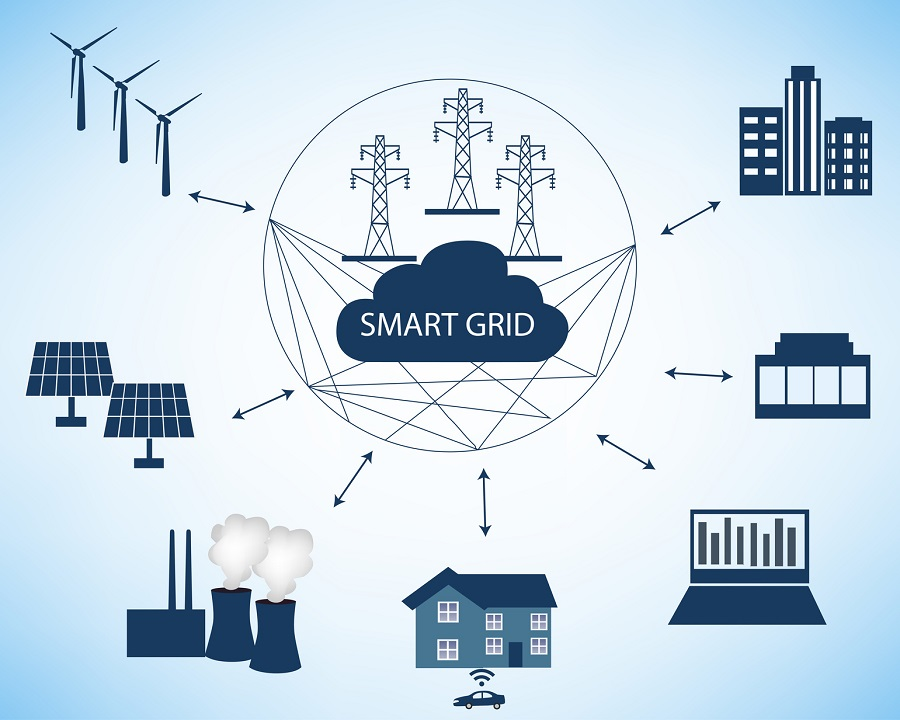
\includegraphics[width=0.75\linewidth]{Intro/smart-grid-2.jpg}
    \caption{Concepto de un smart-grid}
    
\end{figure}
Actualmente, el sistema eléctrico argentino emplea una red tradicional. El proceso desde la generación hasta la distribución está completamente centralizado y engloba casi todo el país en una red única. Como la transición a una smart grid a nivel nacional tardaría varios años (y tampoco está garantizada, siquiera), Solar Link implementa una versión a escala del concepto aprovechando fuentes de energía renovables: en nuestro caso, energía solar.\\

Con una implementación localizada del sistema, Solar Link alterna de manera modular entre el on-grid, que es la red eléctrica común, y el off-grid, que es todo el sistema no conectado a la red principal, lo cual incluye la fuente de energía solar. Al monitorear constantemente los parámetros de consumo generales de la casa, y los consumos provenientes de cada fuente de energía, se puede considerar a Solar Link como un sistema smartgrid.\\

Para completar el esquema de una red inteligente, Solar Link posee conexión a internet, que permitirá al usuario controlar desde su dispositivo los valores de consumo de la casa en el momento, y, utilizando los valores oficiales de tarifas eléctricas, ayudar al consumidor a tomar consciencia de su nivel de consumo y lo que deberá pagar. \\


\subsubsection{Beneficio económico}

Solar Link propone el uso de un sistema solar off-grid, el cual es la alternativa mas económica que se consigue de energía solar. Este sistema consta de panel/es solar/es, batería/s, nuestro cargador MPPT de 3 etapas y un inverter. \\

El sistema que recomendamos instalar en un hogar promedio en Argentina, se compone de dos paneles solares de 380W, un inverter de 2000W, dos baterías de ciclo profundo de 110Ah, el cargador MPPT de 3 etapas de Solar Link, y el módulo Solar Link, con un costo total aproximado de esto ARS \$1.600.000 (USD \$1.600).\\

Mientras tanto, un sistema comparable on-grid, puede salir ARS \$5.000.000 (USD \$5.000). Esto depende del servicio que se contrate y de la empresa que lo realice.\\

No está de más mencionar que al uno producir la energía  que consume, se disminuye el consumo de energía de terceros, el del proveedor eléctrico. Esto quiere decir, que todos los meses se verá reducido el precio que hay que pagar por el suministro de energía eléctrico.\\

El ahorro en este caso no es lineal. Si uno termina consumiendo a fin de mes la mitad de energía que consumiría normalmente, por como funciona el sistema de cobros de las empresas distribuidoras en Argentina, no pagaría la mitad, sino que bastante menos.\\

Esto ocurre porque las empresas establecen un precio para cada KW/h dependiendo de la escala en donde se consuma. Por ejemplo, entre 0KW/h y 200KW/h tiene un precio asignado, entre 200KW/h y 400KW/h otro mayor, y si se exceden esos 400KW/h otro inclusive mayor (estas escalas dependen de la empresa a cargo del suministro eléctrico).\\

Osea, digamos, que cada KW/h entre 0KW/h y 200KW/h valga 1, entre 200KW/h y 400KW/h, 1,5, y si es mayor a 400KW/h, 2. si uno consume 600KW/h, estaría pagando 900, mientras que si uno consume 300KW/h, estaría pagando 350, bastante menos de la mitad. Este ejemplo ilustra como funciona el sistema de cobros de las compañías distribuidoras en Argentina. Las escalas y los valores son a modo de ejemplo. Pueden ser diferentes segun la empresa, la región, y el momento en donde se analice.\\

\subsubsection{Incentivo y concientización}

A través de nuestra aplicación, el usuario tendrá acceso a toda la información que respecta al consumo eléctrico de su casa. Esto le permite conocer al detalle no solo el consumo total, sino tambien el consumo que generó el sistema solar propio.\\

Esto genera en el usuario un sentido de ganancia y de gasto propio. Saber bien cuanto se esta gastando, porque y cuanto de este gasto se amortiguo ayuda a concientizar sobre el consumo de energia en general. \\

Mas allá del gasto de energía, tener un sistema que, ya sea de manera directa o indirecta, ayuda al medio ambiente, tiene un efecto positivo para la psiquis y para el entorno donde uno vive. Saber que uno esta aportando su grano de arena (siendo el mismo economicamente viable y rentable) genera tranquilidad y un sentido de responsabilidad ciudadana. \\

\subsection{Alcance}

Solar Link está destinado principalmente al mercado doméstico argentino, el cual, al día de hoy, está sufriendo de constantes aumentos en la factura de luz. Esto no solo genera un incentivo en el ahorro energético, sino que también convierte a Solar Link en un servicio cada vez mas redituable para el usuario final. \\

Sin embargo, nuestro proyecto tambien puede ser utilizado en cualquier instancia donde se quiera instalar un sistema solar. Puede ser una fábrica, una oficina, un departamento, un quincho, donde se quiera. Los únicos requisitos son tener acceso a la red eléctrica y luz solar a disposición.\\

\subsection{Estado del arte}

Actualmente, en el mercado argentino, existen principalmente tres tipos de instalaciones de energía solar para un hogar. Cada tipo cuenta con sus propias ventajas y desventajas:\\

\begin{table}[H]
\begin{tabular}{|l|l|l|}
\hline
Tipo     & Ventajas                                                                                                                 & Desventajas                                                                                            \\ \hline
On-Grid  & \begin{tabular}[c]{@{}l@{}}Sistema acoplado a la línea doméstica\\ Alimenta casi el 100\% con energía solar\end{tabular} & \begin{tabular}[c]{@{}l@{}}Alto costo\\ Desperdicio de energía\end{tabular}                            \\ \hline
Off-Grid & \begin{tabular}[c]{@{}l@{}}Económico\\ Acumula energía\end{tabular}                                                      & \begin{tabular}[c]{@{}l@{}}Requiere una línea exclusiva \\ para este sistema\end{tabular}              \\ \hline
Híbrido  & \begin{tabular}[c]{@{}l@{}}Sistema acoplado a la línea doméstica\\ Acumula energía\end{tabular}                          & \begin{tabular}[c]{@{}l@{}}Potencia limitada\\ Requiere instalación especial\end{tabular} \\ \hline
\end{tabular}
\end{table}

Los sistemas \textbf{on-grid}, como su nombre lo indica, se instalan directamente en la línea de la casa. Toda la energía que producen los paneles se entregan a la línea general de la casa, sin almacenarse en ningún lado. Si la casa consume mas que lo que generan los paneles, se consume la energía correspondiente a este exceso del proveedor eléctrico, y si consume menos, la energía generada por demás se entrega a la red eléctrica del proveedor. \\

Para este tipo de sistemas es necesaria la instalación de un medidor bidireccional, que mide tanto el consumo de la casa como lo que devuelve por el exceso en la producción. Si bien este medidor descuenta lo que uno devuelve a la red eléctrica, lo que uno consume es mas caro, no es muy redituable y no su instalación depende del proveedor de energía eléctrica.\\

Los sistemas \textbf{off-grid}, por otra parte, acumulan la energía generada por los paneles solares en baterías, para luego convertirla en los 220Vac que necesita la casa. El problema de esto, es que la energía extraída de las baterías no se puede incorporar directamente a la línea de la casa, por lo que es necesario la utilización de una línea exclusiva para lo que este sistema genere. Esto implica tener que hacer una instalación eléctrica aislada e independiente del resto de la casa, algo impráctico si además se tiene en cuenta que la utilización de esta línea debe ser controlada y depende directamente de la carga de los paneles.\\

Los sistemas \textbf{híbridos} son sistemas solares off-grid que se incorporan a la línea de la casa. Pueden utilizar tanto la energía solar acumulada como la energía del proveedor eléctrico. Para utilizar este tipo de sistema es necesaria una instalación especial, que se tiene que realizar en líneas dedicadas. Además, por como es su principio de funcionamiento, el sistema solar no es expandible, por lo que la potencia instalada en un principio no podrá modificarse.\\

Mientras tanto, \textbf{Solar Link} busca recopilar todas las ventajas de estos 3 tipos de sistemas solares, y dejar en el camino todas las desventajas posibles. Se podría decir que Solar Link es un sistema que acumula y utiliza energía solar, acoplado a la línea de la casa, económico, modular expandible y amigable con el usuario, compartiendo toda la información necesaria sobre el sistema solar instalado y el consumo de la casa.

\subsection{Síntesis}
Solar Link aprovecha sus cualidades como gestor inteligente para poder aprovechar la energía solar al máximo. Usualmente, la instalación de una fuente de energía solar por sí sóla no daría abasto para toda la casa (recordemos que en nuestro ejemplo sólo cubría el 30\%), y otros tipos de implementación alternativas a una red inteligente serían rígidas e ineficientes. A través de Solar Link, buscamos que con el control automático de consumo y la separación modular de las redes de la casa logremos maximizar la eficiencia en el consumo, y minimizar los gastos posibles.\\

Nuestro objetivo es introducir al país un sistema capaz de evitar energía cuya generación es, en su mayoría, resultado de fomentar el cambio climático, introduciendo energías renovables y control y concientización del consumo a sus usuarios, en otras palabras un smart grid con energías renovables. Por otro lado, otorga a sus usuarios energía generada por ellos mismos para su hogar, y por lo tanto, no deben pagar por ella. \\

Entre sus beneficios están, el uso de energías renovables, la producción de energía en el propio entorno de uso, que reduciría el consumo en la boleta, una aplicación web que permite ver el consumo y configurarlo, dando control al usuario de su consumo y que sea consciente de este. 